\chapter{Introduction to Neutrino Physics}
\label{c:theoryIntro}

This chapter is aimed at giving an introduction to the physics used in the thesis.

\section{Research Goals}
This research aims to construct a prototype Magnetized Iron Neutrino Detector (Baby MIND) at the European Organization for Nuclear Research (CERN) and understand the performance of the detector to reconstruct charged particle tracks at a test beam at CERN and neutrino interactions with our collaborators in the WAGASCI collaboration at a neutrino beam at the JPARC facility in Japan. This is discussed further in chapter~\ref{c:WAGASCI}.

\section{Theory}\label{section:Theory}
While measuring radioactive beta decay in the first two decades of the 20th century, physicists discovered what was then an anomaly. At the time it was thought that beta decay occurred as a two body process in which a neutron ($n$) decays to a proton ($p$) and electron ($e^-$). If this were the case, the energy of the proton and electron should be discrete and add up to the energy of neutron. However experiments showed that the electron could have a continuous spectrum of energy values, violating the energy conservation law, as seen in \FigRef{fig:betaeng}. In order to solve this anomaly, a third particle, the neutrino ($\nu$), was postulated by Wolfgang Pauli \cite{4Pauli:Online} and then incorporated into the beta decay by Enrico Fermi \cite{5Wilson}. The neutrino was postulated as a neutral particle with mass of less than 1\% of the proton mass and a spin of 1/2. For consistency, the particle being produced in the beta decay was relabelled as the electron antineutrino, $\bar{\nu_e}$, in order to conserve lepton number. The addition of another particle changed the decay to $n \rightarrow p + e^- + \bar{\nu_e}$ and introduced the weak interaction model, as seen in \FigRef{fig:beta}. 

\begin{figure}[h!]
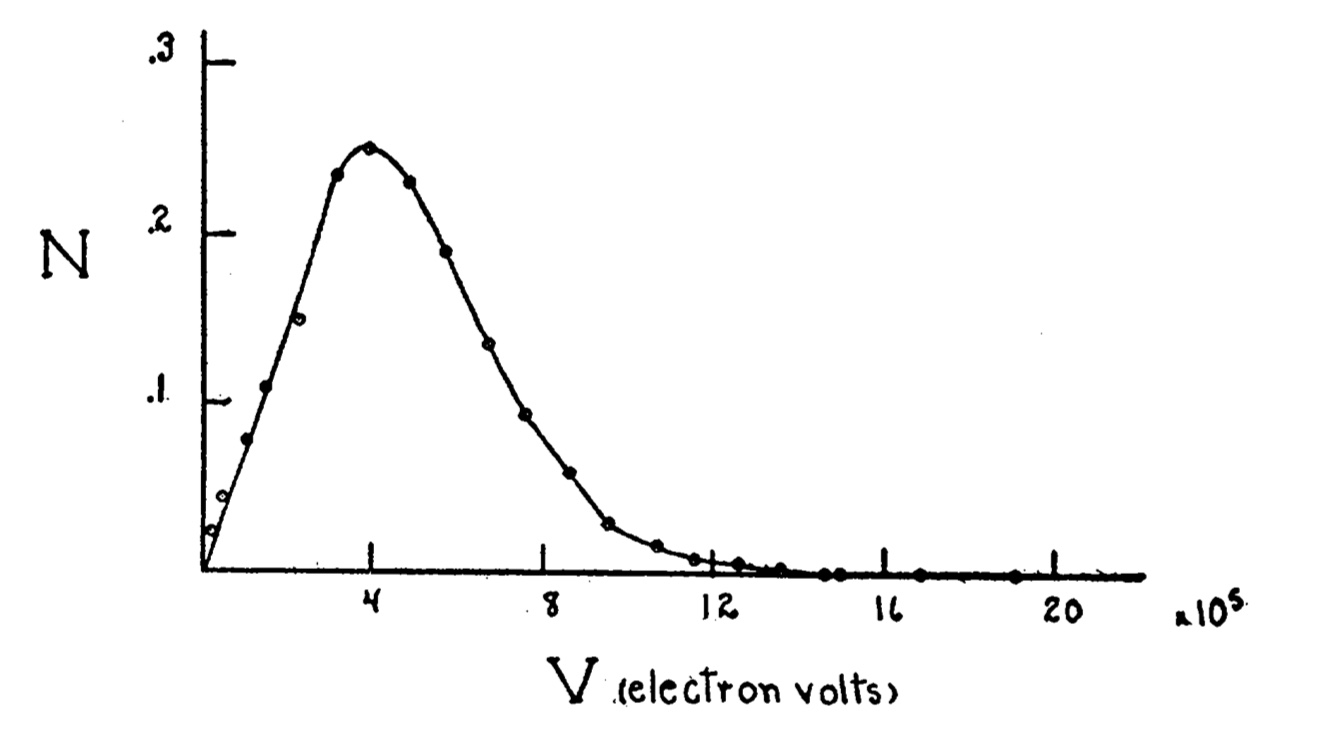
\includegraphics[width=\textwidth]{figures/betaRadium.jpeg}
\caption{The kinetic energy spectrum of the emitted electron from beta decay from a Radium-E source,  \cite{RadiumE}. If no antineutrino were emitted a single electron volt(s) value would be expected.}
 \label{fig:betaeng}
\end{figure}

\begin{figure}[h!]
\centering
\begin{subfigure}{.5\textwidth}
  \centering
  \begin{fmffile}{badBeta}
\begin{fmfgraph*}(120,80)
\fmfstraight
\fmfleft{i1,i2,o1}
\fmfright{o2}

\fmf{fermion}{i1,v1}
\fmf{fermion}{v1,o1}

%fmf{boson}{v1,v2}
\fmf{fermion}{v1,o2}

\fmflabel{n}{i1}
\fmflabel{p}{o1}
\fmflabel{$e^{-}$}{o2}
\end{fmfgraph*}
\end{fmffile}
\vspace{2mm}
  \caption{The initially assumed beta decay}
  %\label{fig:sub1}
\end{subfigure}%
\begin{subfigure}{.5\textwidth}
  \centering
  \begin{fmffile}{beta}
\begin{fmfgraph*}(120,80)
\fmfstraight
\fmfleft{i1,i2,o1}
\fmfright{o2,o3}

\fmf{fermion}{i1,v1}
\fmf{fermion}{v1,o1}

\fmf{boson}{v1,v2}
\fmf{fermion}{v2,o2}
\fmf{fermion}{o3,v2}

\fmflabel{n}{i1}
\fmflabel{p}{o1}
\fmflabel{$e^{-}$}{o2}
\fmflabel{$\bar{\nu}_e$}{o3}
\end{fmfgraph*}
\end{fmffile}
\vspace{2mm}
  \caption{Correct beta decay}
  %\label{fig:sub2}
\end{subfigure}
\vspace{2mm}
\caption{Feynman diagrams showing beta decay.}
\label{fig:beta}
\end{figure}

It would take another twenty years until the neutrino was experimentally discovered by the Savannah river reactor experiment in 1956~\cite{6Reines} which was awarded the Nobel prize in 1995.

After the discovery of the electron neutrino ($\nu_e$), several neutrino experiments were performed and led to the discovery of two other neutrino types/flavours, the muon neutrino ($\nu_\mu$) and the tau neutrino ($\nu_\tau$)~\cite{7Danby, 8Perl, Fix1}.

\subsection{Standard Model neutrino}\label{subsection:SMN}
The Standard Model of particle physics (SM) categorizes all the fundamental particles that have been discovered experimentally and the mathematics of their properties and how they interact \cite{32Burchan:1995, 38griffiths}. 

The particles in SM, seen in \FigRef{fig:standardModel}, can be split into two different types, fermions and gauge bosons, characterised by their half-integer and integer spin. Fermions can be further split depending on their charge, quarks with fractional charge and leptons with integer charge. Gauge bosons are the force mediators for the particle interactions containing the Higgs boson, the only scalar, spin 0, particle in the SM~\cite{35Higgs}.

\begin{figure}[h!]
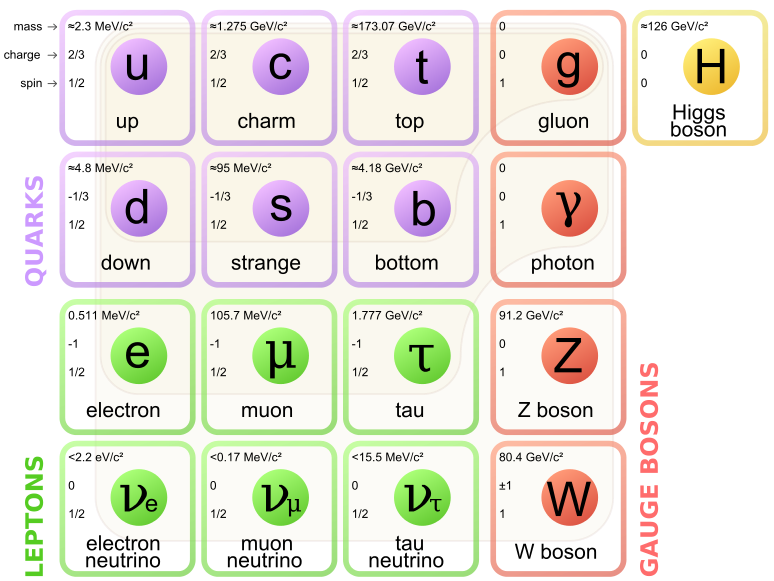
\includegraphics[width=0.7\textwidth]{figures/Standard_Model_of_Elementary_Particles.png}
\caption{The standard model of particle physics where the three first columns represent the so called generations, starting with the first. \cite{33wiki1:Online}}
 \label{fig:standardModel}
\end{figure}

The experiment by \citeauthor{1Helicity} concluded that neutrinos only exist in a left handed chiral state, meaning that momentum and spin are oppositely aligned. They also concluded that anti-neutrinos only exists in the right handed state \cite{1Helicity}. In the initial or unexpanded SM, \cite{34doi:10.1142/9789812562203_0002}, only fermions which have both chiral states have mass through the Brout\hyp{}Englert\hyp{}Higgs mechanism~\cite{35Higgs}. At the time this led to the definition of the neutrino as a massless particle, however in \SubSectionRef{subsection:Neutrinomassandoscillation} it will be shown that neutrino oscillations require at least one of the neutrinos to have mass. This indicates that the SM needs to be extended to account for this new physics.

\subsection{Neutrino interactions}\label{subsection:Neutrino interactions}
%Bitten of too much?Quickly introduce the different parts, center of mass energy, fermi coupling, weinbarg angle and their importance for the comparison.

As discussed previously, neutrino interactions in SM are described by the weak interaction model. Through initial experimental studies, the model was thought to not have any gauge boson and be described by the Lagrangian density $\mathscr{L} = -\frac{G_F}{\sqrt{2}} j_\mu ^\dagger j^\mu$ where $G_F$ is the Fermi constant $\approx 1.17 x 10^{-5} GeV^{-2}$ and $j_\mu$ is the weak V-A current \cite{47Soler}. This gives a good approximation for rates in weak processes but is a non-renormalizable theory. The solution for this is to introduce a massive vector boson drawn in \FigRef{fig:beta} but not yet named as a W boson. Introducing these massive vector bosons leads to some interesting consequences since at this time only Quantum ElectroDynamics (QED) had been described with a non-massive boson, the photon. Introducing the photon into this theory and producing a unified electroweak theory, coupling isospin $g$ and weak hypercharge $g^\prime$, as well as providing the problem of describing how bosons can have mass. It was this unification which was one of the bases of SM and the problem of masses introduces spontaneous symmetry breaking which is part of the Higgs mechanism. In electroweak theory there are in total four bosons, two massive and charged, one massive changeless and one massless and charge less. these are denoted as $W^+, W^-, Z^0, \gamma$. The relationship between the mass of $W$ and $Z^0$ is $m_W = m_Z \cos \theta_W$ where $\theta_W$ is the Weinberg angle.

Neutrino interactions are split into two different parts depending on which boson mediates the interaction.
Charge Current (CC) interactions change the final state quarks or leptons by one unit of electric charge and are mediated by the $W^+$ and $W^-$ bosons while Neutral Current (NC) interactions do not change the charge and are mediated by a $Z^0$ boson. 
To look at possible interactions of neutrinos described in the Standard Model of particle physics, one needs to look at the quantum field theory description of the interactions\cite{3Peskin, 2Hallsjo}. Sample Feynman diagrams showing these interactions can be seen in \FigRef{fig:CC} and \FigRef{fig:NC}.

\begin{figure}[h!]
\centering
\begin{subfigure}{.5\textwidth}
  \centering
  \begin{fmffile}{W+}
\begin{fmfgraph*}(120,80)
\fmfstraight
\fmfleft{i1,i2,o1}
\fmfright{o2,o3}

\fmf{fermion}{v1,i1}
\fmf{fermion}{o1,v1}

\fmf{boson,label=$W^{+}$}{v1,v2}
\fmf{fermion}{o2,v2}
\fmf{fermion}{v2,o3}

\fmflabel{$\bar{d}$}{i1}
\fmflabel{u}{o1}
\fmflabel{$e^{+}$}{o2}
\fmflabel{$\nu_e$}{o3}
\end{fmfgraph*}
\end{fmffile}
  %\caption{A subfigure}
  %\label{fig:sub1}
\end{subfigure}%
\begin{subfigure}{.5\textwidth}
  \centering
  \begin{fmffile}{W-}
\begin{fmfgraph*}(120,80)
\fmfstraight
\fmfleft{i1,i2,o1}
\fmfright{o2,o3}

\fmf{fermion}{i1,v1}
\fmf{fermion}{v1,o1}

\fmf{boson,label=$W^{-}$}{v1,v2}
\fmf{fermion}{v2,o2}
\fmf{fermion}{o3,v2}

\fmflabel{d}{i1}
\fmflabel{$\bar{u}$}{o1}
\fmflabel{$e^{-}$}{o2}
\fmflabel{$\bar{\nu}_e$}{o3}
\end{fmfgraph*}
\end{fmffile}
  %\caption{A subfigure}
  %\label{fig:sub2}
\end{subfigure}
\vspace{2mm}
\caption{Feynman diagrams showing an example of a charge current interaction.}
\label{fig:CC}
\end{figure}

\begin{figure}[h!]
\centering
  \begin{fmffile}{Z}
\begin{fmfgraph*}(120,80)
\fmfstraight
\fmfleft{i1,i2}
\fmfright{o1,o2}

\fmf{fermion}{i1,v1,o1}
%\fmf{fermion}{v1,o1}

\fmf{fermion}{i2,v2,o2}

\fmf{boson,label=$Z^{0}$}{v1,v2}
%\fmf{fermion}{o2,v2}
%\fmf{fermion}{v2,o3}

\fmflabel{$e^{-}$}{i1}
\fmflabel{$\nu_{\mu}$}{i2}
\fmflabel{$e^{-}$}{o1}
\fmflabel{$\nu_{\mu}$}{o2}
\end{fmfgraph*}
\end{fmffile}
  %\caption{A subfigure}
  %\label{fig:sub1}

\vspace{2mm}
\caption{Feynman diagram showing an example of a neutral current interaction.}
\label{fig:NC}
\end{figure}

From the Feynman diagrams one can calculate the probability of the interaction occurring, details can be found in \cite{3Peskin}. 

It is interesting to compare the probability for Charge Current and Neutral Current interactions with the equivalent QED or electromagnetic interactions. In  \FigRef{fig:weakQED} a comparison is made between QED and a weak interaction with the same initial and final states. Calculating the cross-sections when $E<<M_Z$ the following quotient is produced: $\frac{\sigma_{Weak}}{\sigma_{QED}} \approx (\frac{s}{M_Z^2})^2$ where s is the square of the center of mass energy, $M_Z$ is the mass of the Z-boson. Currently the Z-boson mass is $91.1876 GeV$~\cite{13PDG} but since s varies it is hard to give a value to the quotient. For the energy range where $E<<M_Z$ this quotient varies from $0.01 \rightarrow 0.1225$. With the current values QED is approximately 100 times more likely to occur than a weak interaction..

\begin{figure}[h!]
\centering
\begin{subfigure}{.5\textwidth}
  \centering
  \begin{fmffile}{QED}
\begin{fmfgraph*}(120,80)
\fmfstraight
\fmfleft{i1,i2,o1}
\fmfright{o2,o3}

\fmf{fermion}{v1,i1}
\fmf{fermion}{o1,v1}

\fmf{boson,label=$\gamma$}{v1,v2}
\fmf{fermion}{o2,v2}
\fmf{fermion}{v2,o3}

\fmflabel{$e^{+}$}{i1}
\fmflabel{$e^{-}$}{o1}
\fmflabel{$\bar{f}$}{o2}
\fmflabel{$f$}{o3}
\end{fmfgraph*}
\end{fmffile}
  %\caption{A subfigure}
  %\label{fig:sub1}
\end{subfigure}%
\begin{subfigure}{.5\textwidth}
  \centering
  \begin{fmffile}{Weak}
\begin{fmfgraph*}(120,80)
\fmfstraight
\fmfleft{i1,i2,o1}
\fmfright{o2,o3}

\fmf{fermion}{v1,i1}
\fmf{fermion}{o1,v1}

\fmf{boson,label=$Z^0$}{v1,v2}
\fmf{fermion}{o2,v2}
\fmf{fermion}{v2,o3}

\fmflabel{$e^{+}$}{i1}
\fmflabel{$e^{-}$}{o1}
\fmflabel{$\bar{f}$}{o2}
\fmflabel{$f$}{o3}
\end{fmfgraph*}
\end{fmffile}
  %\caption{A subfigure}
  %\label{fig:sub2}
\end{subfigure}
\vspace{2mm}
\caption{The QED and the weak contributions to the scattering electron-positron to any quark or lepton pair.\protect\footnotemark}
\label{fig:weakQED}
\end{figure}
\footnotetext{If $f=e^-$ a T-channel diagram has to be added as well} 

The CC and NC examples in  \FigRef{fig:CMPNCCC} with electrons and muon neutrinos, so that the final states can be distinguished, the cross sections of both can be written as $\sigma_{CC} (\nu_\mu e^-) \approx \frac{G_F^2 s}{\pi} $ and $\sigma_{NC} (\nu_\mu e^-) \approx \frac{G_F^2 s}{\pi} \left[ (-\frac{1}{2} + \sin^2 \theta_W)^2 + \frac{1}{3}\sin^4 \theta_W\right] $ where $G_F$ is the Fermi coupling constant and $\theta_W$ is the Weinberg angle. This gives a relation CC and NC as $\frac{\sigma_{CC}}{\sigma_{NC}} = 1/\left[ (-\frac{1}{2} + \sin^2 \theta_W)^2 + \frac{1}{3}\sin^4 \theta_W\right] \approx 11$. With the current values CC is approximately 11 times more likely to occur than NC.

\begin{figure}[h!]
\centering
\begin{subfigure}{.5\textwidth}
  \centering
  \begin{fmffile}{ECC}
\begin{fmfgraph*}(120,80)
\fmfstraight
\fmfleft{i1,i2}
\fmfright{o1,o2}

\fmf{fermion}{i1,v1,o1}
%\fmf{fermion}{v1,o1}

\fmf{fermion}{i2,v2,o2}

\fmf{boson,label=$W^-$}{v1,v2}
%\fmf{fermion}{o2,v2}
%\fmf{fermion}{v2,o3}

\fmflabel{$e^{-}$}{i1}
\fmflabel{$\nu_{\mu}$}{i2}
\fmflabel{$\nu_{e}$}{o1}
\fmflabel{$\mu^-$}{o2}
\end{fmfgraph*}
\end{fmffile}
  %\caption{A subfigure}
  %\label{fig:sub1}
\end{subfigure}%
\begin{subfigure}{.5\textwidth}
  \centering
  \begin{fmffile}{ENC}
\begin{fmfgraph*}(120,80)
\fmfstraight
\fmfleft{i1,i2}
\fmfright{o1,o2}

\fmf{fermion}{i1,v1,o1}
%\fmf{fermion}{v1,o1}

\fmf{fermion}{i2,v2,o2}

\fmf{boson,label=$Z^{0}$}{v1,v2}
%\fmf{fermion}{o2,v2}
%\fmf{fermion}{v2,o3}

\fmflabel{$e^{-}$}{i1}
\fmflabel{$\nu_{\mu}$}{i2}
\fmflabel{$e^-$}{o1}
\fmflabel{$\nu_{\mu}$}{o2}
\end{fmfgraph*}
\end{fmffile}
  %\caption{A subfigure}
  %\label{fig:sub2}
\end{subfigure}
\vspace{2mm}
\caption{Feynman diagrams, CC(Left) and NC(Right) with the same initial states.}
\label{fig:CMPNCCC}
\end{figure}

\subsection{Missing neutrinos}\label{subsection:Missing}

Stars generate energy principally through the proton–proton chain reaction \cite{48Solar}. In this chain electron neutrino are produced through proton-proton interactions and beta decay processes. 
\begin{equation}
\label{eq:ppreaction}
H^+ + H^+ \rightarrow ^2_2He \rightarrow ^2H + e^+ + \nu_e
\end{equation}
The proton-proton interaction has the highest flux, $6.1 x 10^10 cm^{-2} sec^{-1}$ but produces neutrinos at very low energies  (<0.4 MeV) making them difficult to detect. 
Further on in this chain a Boron decay,
\begin{equation}
\label{eq:BoronDecay}
^8_5B \rightarrow ^9_4 Be + e^+ + \nu_e
\end{equation}
produces electron neutrinos with energies up to 14 MeV, however the fluxes are much lower than proton-proton interactions, $3.2 x 10^6 cm^{-2} sec^{-1}$. Neutrinos in this energy can be used in inverse-beta decay transforming chlorine into argon.
\begin{equation}
\nu_e + ^37 Cl \rightarrow ^37 Ar + e^-
\end{equation}
The amount of argon can then be counted and related to the neutrino flux.

The Homestake experiment used this technique ran from 1970 until 1994 with a goal to measure the flux of electron neutrinos. They measured the flux of electron neutrinos and found only around 1/3, (1.75/4.7), of the expected value from the theoretical model of the nuclear reactions in the core of the sun \cite{9Davis}. The discussion arose as to what was wrong, the theoretical solar model or the experiment. One of the possible explanations for the deficit was neutrino oscillations proposed by Bruno Pontecorvo~\cite{11Pontecorvo}. This theory was later verified at both the Sudbury Neutrino Observatory (SNO)~\cite{Fix6} and Super-Kamiokande~\cite{10Fukuda}. All three experiments were awarded Nobel prizes and have paved the way for physics beyond the Standard Model.

\subsection{Neutrino mass and oscillation in vacuum}\label{subsection:Neutrinomassandoscillation}
While looking at an analog of neutral kaon mixing for neutrinos Bruno Pontecorvo, in 1957, developed the concept of neutrino-antineutrino transitions~\cite{11Pontecorvo}. Even though to date no matter-antimatter oscillation had been observed, the concept formed the foundation of lepton mixing, which was developed by Maki, Nakagawa, and Sakata~\cite{12Maki} and refined into a neutrino flavour oscillation model by Bruno Pontecorvo. They managed to show that neutrino mixing is a natural outcome of adding neutrino mass to a gauge theory~\cite{11Pontecorvo}

The relation between the flavour and mass eigenstates can be expressed as,
\begin{equation}
\label{eq:eigenstates}
 \left| \nu_\alpha \right\rangle = \sum_{i} U^{*}_{\alpha i} \left| \nu_i \right\rangle,
 \left| \bar{\nu_\alpha} \right\rangle = \sum_{i} U_{\alpha i} \left| \bar{\nu_i} \right\rangle\
 \end{equation}
where
 $\left| \nu_\alpha \right\rangle $ is a neutrino with a fixed flavour, $\alpha$ is one of \{e,$\mu$,$\tau$\} and  $\left| \nu_i \right\rangle$ is a neutrino with a fixed mass.
$U$ is the Pontecorvo-Maki-Nagawa-Sakata (PMNS) matrix in \eqref{PMNS},
\begin{equation}
\label{PMNS}
\begin{aligned}
U ={} & 
 \begin{pmatrix}
 c_{12} & s_{12} & 0\\
  -s_{12} & c_{12} & 0\\
  0 & 0 & 1\\
 \end{pmatrix} 
  \begin{pmatrix}
 1 & 0 & 0\\
  0 & c_{23} & s_{23}\\
  0 & -s_{23} & c_{23}\\
 \end{pmatrix} 
   \begin{pmatrix}
 c_{13} & 0 & s_{13}e^{i\delta_{CP}}\\
  0 & 1 & 0\\
  -s_{13}e^{-i\delta_{CP}} & 0 & c_{13}\\
 \end{pmatrix} 
 \\
 & \times
  \begin{pmatrix}
1 & 0& 0\\
  0 & e^{i\phi_2} & 0\\
  0 & 0 & e^{i\phi_3}\\
 \end{pmatrix} 
 \end{aligned}
\end{equation}
where $s_{ij} = \sin\theta_{ij}$ and $c_{ij} = \cos\theta_{ij}$ with $\theta_{ij}$ the three mixing angles and $\delta_{CP}$, $\phi_2$ and $\phi_3$ are complex phases. The parameters $\phi_2$ and $\phi_3$ are only non-zero if neutrinos are their own antiparticles, which is still unknown at the time of writing this~\cite{13PDG}.

The probability of finding a neutrino in a specific time-dependent state is related to the mass states through the PMNS matrix elements and the time-evolution operator. The PMNS introduces a rotation in the space of mass eigenstates. The derivations of the oscillation probability for two-neutrino and three-neutrino oscillations can be found in the literature \cite{34doi:10.1142/9789812562203_0002}. The three neutrino flavour state shown in equation \ref{eq:eigenstates} evolves as a function of time as:
%The interpretation is similar to that of a time-dependent quantum state, the probability of finding a neutrino in a specific state is related to the mass states through the PMNS matrix in which the elements are time dependent.
%It can also be thought of as a rotation in space. The derivations of the oscillation probability for assuming only two neutrinos and also for three neutrinos are often given in literature for instance it is given in . The three neutrino flavour state \ref{eq:eigenstates} in an initial beam evolves in time as:

\begin{equation}
\label{eq:eigenstatesTime}
 \left| \nu_\alpha (t) \right\rangle = \sum_{i} e^{-i E_i t} U_{\alpha i} \left| \nu_i \right\rangle\,
 \end{equation}

which gives the probability of flavour evolution as 
\begin{equation}
\begin{aligned}
P_{\nu_\alpha \rightarrow \nu_\beta} (t) &= \left|  \langle \nu_\beta \left| \nu_\alpha     \right\rangle  \right|^2
& = \sum_{i,j} \left| U_{\alpha i} U_{\beta i}^* U{\alpha j}^* U_{\beta j} \right| \cos[(E_i - E_j)t -arg(U_{\alpha i} U_{\beta i}^* U{\alpha j}^* U_{\beta j} ) ]
\end{aligned}
\end{equation}

\begin{equation}
\label{eq:Energy-momentum}
E_\alpha = \sqrt{\vec{p}^2 + m_i^2} \approx \left| \vec{p} \right| + \frac{m_i^2}{2\left| \vec{p} \right|}
\end{equation}

If one has a beam of neutrinos in an initial flavour state $\|\nu_\alpha \rangle$, the probability to find the neutrinos changing to flavour state $\|\nu_\beta \rangle$, after a distance $x$, is given by
%Which can then be rewritten to depend on distance travelled by the beam (x) if using a relativistic approximation of the   as

\begin{equation}
\label{eq:Problength}
\begin{aligned}
P_{\nu_\alpha \rightarrow \nu_\beta} (x) &= \left|  \langle \nu_\beta \left| \nu_\alpha     \right\rangle  \right|^2
& = \sum_{i,j} \left| U_{\alpha i} U_{\beta i}^* U{\alpha j}^* U_{\beta j} \right| \cos[\frac{2\pi x}{L_{ij}} -arg(U_{\alpha i} U_{\beta i}^* U_{\alpha j}^* U_{\beta j} ) ],
\end{aligned}
\end{equation}
where the approximate energy-momentum relationship of equation \ref{eq:Energy-momentum} has been taken into account, with where the oscillation length given by $L_{ij} = \frac{4\pi  \left| \vec{p} \right| }{\left| m_i^2 - m_j^2 \right|}$ and $\vec{p}$ is the 3-momentum of the neutrinos in the initial beam.

The mass-squared difference between neutrino mass states $\left|m_i^2 - m_j^2\right|$ has to be different to zero for there to be neutrino oscillations, so at least one of the neutrinos must have non-zero mass which currently is not explained through the Standard Model. Furthermore, if the elements of the PMNS matrix $U_{\alpha i}$ are all real then $arg(U_{\alpha i} U^*_{\beta i} U^*_{\alpha j}  U_{\beta i} ) = 0$ and the CP-violating phase $\delta_{CP} =0$. Current experimental focus lies with trying to measure values for all of these parameters. .

Looking at the oscillation probability \eqref{eq:Problength} two main classes of experiments for neutrino oscillations can be devised. Finding a distance x to the source where $P_{\nu_\alpha \rightarrow \nu_\alpha} (x) < 1$ it is possible to look at so called disappearance of the beam by comparing the expected neutrino flux to the observed. For the disappearing flavour there must be a probability, $P_{\nu_\alpha \rightarrow \nu_\beta} (x) > 0, \alpha=\beta$ for another flavour to appear. The second kind of experiment, denoted as appearance, is based on looking for interaction products which are impossible without oscillations.  An example of this would be to see a positron from a muon neutrino beam. More on this can be found well described in~\cite{34doi:10.1142/9789812562203_0002} and examples of different detectors will be discussed in chapter~\ref{c:expIntro}.

Charge conjugation and parity (C and P, CP) symmetry states that physics should be the same for particles and anti-particles while the spatial coordinates are inverted. If $\delta_{CP}$ is non-zero it would imply CP symmetry is violated it would imply a difference between the rate of neutrino and anti-neutrino oscillations and could be responsible for the matter-antimatter asymmetry of the early universe. Current best-fit values have $\delta_{CP} = -1.791$ for normal mass ordering and $\delta_{CP} = -1.414$ for inverted mass ordering\cite{T2KResults}.

%Also that if $U_{\alpha i}$ is real, which is related to $\delta_{CP} = 0$, then $arg(U_{\alpha i} U_{\beta i}^* U_{\alpha j}^* U_{\beta j} ) = 0$.
%It can be seen that if $m_i^2 - m_j^2 = 0 $ this probability becomes $0$ which contradicts the experimental results. This means that atleast one of the neutrinos 

%and one of the most interesting for understanding more about the Big Bang theory is the complex phase $\delta_{CP}$. This is known as the CP-violating phase which, if non-zero, would state that there is a difference between how normal and anti-neutrinos oscillate. \textbf{Experimental value so far of CP}

Table \ref{table:UpperNMass} provides the current mass limits for neutrinos, note that currently there is no lower limit since it is only known that at least two of the neutrinos must have mass.

\begin {table}[H]
\begin{center}
\begin{tabular}{ |c|c|c| } 
 \hline
 Particle & 95\% CL Mass limit (MeV) & 95\% CL Anti-particle mass limit (MeV) \\ 
  \hline
 $\nu_e$ & $<0.225$ & $<2 \cdot 10^{-3}$ \\ 
 $\nu_\mu$ & $<0.19$ & No Data \\ 
  $\nu_\tau$ & $< 18.2$ & No Data \\ 
 \hline

\end{tabular}
\end{center}
\caption{Current upper neutrino mass limits ~\cite{13PDG}}
\label{table:UpperNMass}
\end {table}

\subsection{CP-violation, baryogenesis and leptogenesis}
According to the Big Bang theory, matter and anti-matter were created in equal amounts\cite{14Berry}. Through observations of the universe, much more matter has been found compared to anti-matter. This provided one of the major unsolved problems in physics, where is all the anti-matter? There has currently not been any sign of an annihilation horizon, where matter and anti-matter interact nor has there been any sign of this in the cosmic background radiation\cite{14Berry}. One direct measurement was AMS-01, (Alpha Magnetic Spectrometer),which measured the ratio of anti-helium to helium in the universe to be of the order of $10^{-6}$~\cite{15AMS1}. 

The follow-up experiment, AMS-02, which is operational in the International Space Station, confirmed these results and measured the antibaryon component of the universe to be $\sim 10^{-9}$ less that of baryons~\cite{16AMS2}. As of now our current models account this difference to be $O(1)$ thus a factor of $10^9$ too small\cite{49Matter}. To properly account for the difference thus there must be unknown processes that account for this.

There exist two approaches to explain the matter asymmetry of the universe. The first is baryogenesis which studies possible mechanisms to enhance the baryon-antibaryon asymmetry, and the second is leptogenesis, in which CP violation in leptons translates into a baryon asymmetry. Leptogenesis will be covered in this thesis as it relates to neutrinos also it should be added that there are theories which explain baryogenesis through leptogenesis.

If neutrinos violate CP by their oscillations being different for neutrinos and anti-neutrinos, this could explain the matter anti-matter imbalance that has been observed. CP-violation exists in the Standard Model but it cannot explain the observed difference~\cite{3Peskin}, and measurements of the CP-violation in neutrino oscillations have not yet been able to show any conclusive results~\cite{17Gonzalez}.

\subsection{Current theory of leptogenesis}
Andrei Sakharov proposed three necessary conditions that any baryon-generating interaction, which would produce matter antimatter imbalance, must satisfy~\cite{37Sakharov}. These conditions are:
\begin{itemize}
\item Baryon number violation.
\item C-and CP-violation.
\item Deviation from thermal equilibrium.
\end{itemize}

The first conditions is very important in that it related cosmological models with models in particle physics. It also gives us a way to produce an excess of baryons over anti-baryons, as long as there is no reverse interaction, hence requiring the C violation. CP-violation is needed to counteract the balancing as well and finally out of thermal equilibrium to get around CPT-symmetry. As briefly mentioned previously the second condition is fulfilled in the SM, but not enough, and the third can always be satisfied.

In \cite{36CRC} a number of viable scenarios for baryogenesis are briefly discussed, for instance Grand Unified theories, heavy Majorana neutrinos and supersymmetry.

\section{Current Theories to explain neutrino mass}
As discussed in subsection~\ref{subsection:SMN}, it is clear that without having both types of chiral, neutrinos cannot have mass through Brout\hyp{}Englert\hyp{}Higgs mechanism~\cite{35Higgs}. Currently there are two different approaches to explain the neutrino masses through processes which already exist in the SM by implying that some observations still have to be made.

\subsection{Dirac neutrinos}
Are their heavier neutrinos with the other chirality which have yet to be discovered? If this is the case then neutrinos can have mass through the Brout\hyp{}Englert\hyp{}Higgs mechanism. This is what was used by MNS for the PMNS matrix.

\subsection{Majorana neutrinos}



If they are neutral, thus anti and normal are the same particle. (Z boson mass) only chirality would distinguish them.



Because antineutrinos and neutrinos are neutral particles, it is possible that they are the same particle. Particles that have this property are known as Majorana particles, after the Italian physicist Ettore Majorana who first proposed the concept.
 For the case of neutrinos this theory has gained popularity as it can be used, in combination with the seesaw mechanism, to explain why neutrino masses are so small compared to those of the other elementary particles, such as electrons or quarks. 
 
 Majorana neutrinos have the property that the neutrino and antineutrino could be distinguished only by chirality; what experiments observe as a difference between the neutrino and antineutrino could simply be due to one particle with two possible chiralities.

For example, if neutrinos are indeed Majorana particles, then lepton-number violating processes such as neutrinoless double beta decay would be allowed

\subsection{Seesaw mechanism}







%\subsection{Neutrinoless double beta decay}
%This experiment can conclusively show that neutrinos must be majorana particles. Reference? How? Diagrams

%\section{Extended theories with neutrinos}
%In this section some extended theories requiring more neutrinos or neutrinolike particles are presented.



%\subsection{Massive neutrinos as dark matter}
%What is SUSY? What is a neutralio? Sterile neutrinos

%What is dark matter? Why cold? Current ideas and theories? How does it relate to neutrinos? Or to neutralinos?

%==============================================================================
%\section{Thesis Statement}
%\label{c:intro:thesisstatement}

%This is a thesis statement. There are many like it, but this one is mine.


